%% AMS-LaTeX Created by Wolfram Mathematica 9.0 : www.wolfram.com

\documentclass{article}
\usepackage{amsmath, amssymb, graphics, setspace}
\usepackage{graphicx}

\usepackage[utf8]{inputenc}
\usepackage{spverbatim}
\usepackage{geometry}
 \geometry{
 a4paper,
 left=15mm,
 right=10mm,
 top=20mm,
 bottom=20mm,
 }



\newcommand{\mathsym}[1]{{}}
\newcommand{\unicode}[1]{{}}

\newcounter{mathematicapage}
\begin{document}


\section{Sound waves}

\paragraph{sound eq}

initial
$v_0 = 0, \rho_0 , p_0$




perturbations ($p\prime, \rho\prime, v$)

$ p = p_0 + p\prime $

$ \rho = \rho_0 + \rho\prime $

Cont eq lin:

$ \frac{\partial \rho\prime}{\partial t} + \rho_0 \nabla \cdot v = 0 $

Euler lin:

$ \frac{\partial v}{\partial t} + \frac{1}{\rho_0} \nabla p\prime = 0 $


def: 

$c_s = \big( \frac{\partial p}{\partial \rho}\big)_s$



energy eq: adiabatic process:


$p\prime = c_s^{2} \rho\prime$

$\implies$




\subsection{sound equation in inhomogeneous}

$\frac{\partial}{\partial t} \big(\frac{1}{c_s^{2}(x,t)} \frac{\partial p}{\partial t}\big) = \nabla^{2} p    $

Time independent:

$\frac{1}{c_s^{2}(x)} \frac{\partial^{2} p}{\partial t^{2}} = \nabla^{2} p    $

\paragraph{Eikonal solution approx}


$p(x,t) = a(x,t) e^{i \phi(x,t)}$

Notations:

$\omega(x,t) = -\frac{\partial \phi}{\partial t}$

$k(x,t) = -\nabla \phi$


Reemplazano p en la ecuación y definiendo $c_g = \frac{\partial \omega}{\partial k}$ :

$\omega^{2} = c_s^{2} k^2$

$\frac{\partial a}{\partial t} + c_g \cdot \nabla a = -\frac{1}{2} \frac{a}{|k| c_s} (\frac{\partial \omega}{\partial t} + c_s^{2} \cdot \nabla k) $


$\implies $



$\frac{\partial \omega}{\partial t} + c_g \cdot \nabla \omega = 0 $

$\frac{\partial k}{\partial t} + c_g \cdot \nabla k = -k \cdot \nabla c_g $

Energy conservation:

$\frac{\partial E}{\partial t} + c_g \cdot \nabla E = -E \nabla \cdot c_g $


$E(x,t) = \frac{|a|^{2}}{\rho_0 c_s^{2}} $

1D ($c_s = c_g$):

$\frac{\partial k}{\partial t} + c_s \frac{\partial k}{\partial x} = -c_s $

$\frac{\partial \omega}{\partial t} + c_s \frac{\partial \omega}{\partial x} = 0 $

$\frac{\partial k}{\partial t} + c_s \frac{\partial k}{\partial x} = -k \frac{\partial c_s}{\partial x} $

$\frac{\partial E}{\partial t} + c_s \frac{\partial E}{\partial x} = -E \frac{\partial  c_s}{\partial x} $




rays characterictics method:

para un rayo (trayectoria):

solución de la la ecuación 

$\frac{dx}{dt} = c_s $

$ x_p(t) , x_p(0) = x_p $

def

$\omega_p(t) = \omega(x_p(t), t)$

$k_p(t) = k(x_p(t), t)$

$a_p(t) = a(x_p(t), t)$




$\frac{d\omega_p}{dt} = 0$

$\frac{dk_p}{dt} = -k_p \frac{\partial c_s}{\partial x} (x_p(t))$





$\frac{dc_s}{dt}  =  \frac{\partial c_s}{\partial x}(x_p(t)) c_s$

$\implies $

$\frac{dk_p}{dt} = -k_p  \frac{1}{c_s} \frac{dc_s}{dt}$

$\implies $

$\frac{dln(k_p)}{dt} = - \frac{dln(c_s)}{dt}$

$\implies $

$ k(x_p(t), t)  cs(x_p(t)) = constant $

$ E(x_p(t), t)  cs(x_p(t)) = constant $ 

$ \omega(x_p(t), t)  = constant $


v, p solutions in WKB approx (con amplitudes V y P)
(
$v = V e^{i\phi} $
$p = P e^{i\phi} $
)

introducimos

$\rho\prime \frac{\partial v}{\partial t} = - \nabla p\prime$




$\frac{\rho_0 |V|^{2}}{2} = \frac{|P|^{2}} {2 \rho_0 c_s^{2}} $


$\implies$

$E = \frac{|A|^{2}}{\rho_0 c_s^2} $









\section{Transf fourier}

Salida de mathematica de la integral de la transf fourier:

\begin{spverbatim}

$Assumptions = {Element[{k0,z0,zf,zc,W}, Reals], k0>0, z0>0, zf >0 , zf >0, zc >0, W>0 }
Print[FullSimplify[Integrate[Exp[- (z-zc)^2 / W^2] Cos[2 Pi  k0 (z - z0)/ (zf - z0)] Exp[- 2 Pi I m z / (zf - z0)],  {z, -Infinity, Infinity} ]]]

\end{spverbatim}

$
f1(m)=F( \frac{2\pi m}{z_f - z_0} ) = \int_{- \infty}^{\infty}{e^{-\frac{(z-z_c)^2}{W^2}} cos(\frac{2 \pi k_0 (z-z_0)}{z_f - z_0}) e^{-\frac{2 \pi i m z }{z_f - z_0}} dz } = $

$\frac{1}{2} e^{-\frac{\pi  \left(\text{$k_0$}^2 \pi  W^2+m \left(m \pi  W^2-2 i \text{$z_c$} (\text{$z_0$}-\text{$z_f$})\right)+2 \text{$k_0$} \left(m \pi  W^2+i
(\text{$z_0$}+\text{$z_c$}) (\text{$z_0$}+\text{$z_f$})\right)\right)}{(\text{$z_0$}-\text{$z_f$})^2}} \left(e^{\frac{4 i \text{$k_0$} \pi  \text{$z_0$} (\text{$z_c$}+\text{$z_f$})}{(\text{$z_0$}-\text{$z_f$})^2}}+e^{\frac{4
\text{$k_0$} \pi  \left(m \pi  W^2+i \left(\text{$z_0$}^2+\text{$z_c$} \text{$z_f$}\right)\right)}{(\text{$z_0$}-\text{$z_f$})^2}}\right) \sqrt{\pi } W$


Salida de FourierTransform mathematica con FourierParameters 0, -2$\pi$ 

\begin{verbatim}

$Assumptions = {Element[{k0,z0,zf,zc,W}, Reals], k0>0, z0>0, zf >0 , zf >0, zc >0, W>0 }
h[z_, k0_, z0_, zf_, zc_, W_]:= Exp[-(z-zc)^2/W^2] Cos[2 Pi k0 (z - z0) / (zf - z0) ]
Print[FullSimplify[FourierTransform[h[z, k0, z0, zf, zc, W], z, k, FourierParameters->{0,-2 Pi}]] ]

\end{verbatim}
$f2(k)=$

$\frac{1}{2} \left(e^{-\frac{\pi  \left(\text{$k_0$}^2 \pi  W^2-2 \text{$k_0$} \left(k \pi  W^2-i \text{$z_0$}+i \text{$z_c$}\right) (\text{$z_0$}-\text{$z_f$})+k
\left(k \pi  W^2+2 i \text{$z_c$}\right) (\text{$z_0$}-\text{$z_f$})^2\right)}{(\text{$z_0$}-\text{$z_f$})^2}}+ \\
e^{-\frac{\pi  \left(\text{$k_0$}^2 \pi  W^2+2 \text{$k_0$}
\left(k \pi  W^2-i \text{$z_0$}+i \text{$z_c$}\right) (\text{$z_0$}-\text{$z_f$})+k \left(k \pi  W^2+2 i \text{$z_c$}\right) (\text{$z_0$}-\text{$z_f$})^2\right)}{(\text{$z_0$}-\text{$z_f$})^2}}\right)
\sqrt{\pi } W$

En esta reemplazo k = k / (zf - z0) y los graficos salen iguales ($f1(k) = f2(\frac{k}{z_f - z0})$)


Ademas la salida de:
\begin{spverbatim}
$Assumptions = {Element[{k0,z0,zf,zc,W}, Reals], k0>0, z0>0, zf >0 , zf >0, zc >0, W>0 }

f1[m_]:=((E^(((4*I)*k0*Pi*z0*(zc + zf))/(z0 - zf)^2) + E^((4*k0*Pi*(m*Pi*W^2 + I*(z0^2 + zc*zf)))/(z0 - zf)^2))*Sqrt[Pi]*W)/
  (2*E^((Pi*(k0^2*Pi*W^2 + m*(m*Pi*W^2 - (2*I)*zc*(z0 - zf)) + 2*k0*(m*Pi*W^2 + I*(z0 + zc)*(z0 + zf))))/(z0 - zf)^2))
f2[k_]:=((E^(-((Pi*(k0^2*Pi*W^2 - 2*k0*(k*Pi*W^2 - I*z0 + I*zc)*(z0 - zf) + k*(k*Pi*W^2 + (2*I)*zc)*(z0 - zf)^2))/(z0 - zf)^2)) +
      E^(-((Pi*(k0^2*Pi*W^2 + 2*k0*(k*Pi*W^2 - I*z0 + I*zc)*(z0 - zf) + k*(k*Pi*W^2 + (2*I)*zc)*(z0 - zf)^2))/(z0 - zf)^2)))*Sqrt[Pi]*W)/2

Print[FullSimplify[f1[k]-f2[k/(zf-z0)]]]

\end{spverbatim}

es 0


Elijo f2 forma para simplificar (después de hacer los gráficos de los modulos de los valores de la función , tal como imaginaba la primera exponencial corresponde a la gaussiana de las frecuancias negativas y la segunda de las frequencias positivas):


$f1(k) = f2(\frac{k}{(z_f - z_0)}) = $

$ \frac{W \sqrt{\pi}}{2}  (e^{-\frac{\pi (k_0^2 \pi  W^2 + 2 k_0 k \pi W^2 + 2 k_0 i  (z_c - z_0) (z_f-z_0)+k^2 \pi W^2 +
2 i k z_c (z_f - z_0))}{(z_0-z_f)^2}}+e^{-\frac{\pi  (k_0^2 \pi  W^2 - 2 k_0 k \pi  W^2 - 2 k_0 i (z_c - z_0) (z_f-z_0)+k^2 \pi  W^2+2 i k z_c (z_f - z_0))}{(z_0-z_f)^2}}) =
$

$ \frac{W \sqrt{\pi}}{2}  (e^{-\frac{\pi \big[ \pi  W^2 (k + k_0)^2   + 2 k_0 i z_c(z_f - z_0)   - 2 k_0 i z_0 (z_f-z_0) +
2 i k z_c (z_f - z_0)\big]}{(z_0-z_f)^2}}+e^{-\frac{\pi \big[\pi  W^2 (k - k_0)^2  -2 k_0 i z_c(z_f - z_0)  + 2 k_0 i z_0 (z_f-z_0)+2 i k z_c (z_f - z_0)\big]}{z_0-z_f)^2}}) =
$

$ \frac{W \sqrt{\pi}}{2}  (e^{-\frac{\pi \big[ \pi  W^2 (k + k_0)^2   + 2  i z_c(z_f - z_0)(k_0 + k)   - 2 k_0 i z_0 (z_f-z_0) \big]}{(z_0-z_f)^2}}+e^{-\frac{\pi \big[\pi  W^2 (k - k_0)^2  +2 i z_c(z_f - z_0)(k - k_0)  + 2 k_0 i z_0 (z_f-z_0)\big]}{(z_0-z_f)^2}}) =
$

Considerando $z_c$ = 0 
las exponenciales son  gaussianas  con w = $\frac{z_f - z_0}{\pi W}$ la primera centrada en $-k_0$ y la segunda en $k_0$
y cuando calculamos el modulo las constantes $ abs(exp( - 2 k_0 i z_0 (z_f-z_0))) = abs(exp( 2 k_0 i z_0 (z_f-z_0)))  = 1$
y la amplitud queda $\frac{W \sqrt{\pi}}{2}$ igual que se ve en el gráfico (con valores :  z0=3.100, zf = 7.400, k0 = 60, zc = 3.745, W = 0.050) : con rojo había hecho el plot de la función entera y con verde y azul de las 2 partes al principio para estar segura que correspondían a las 2 partes

\begin{figure}[!ht] 
 \centering 
 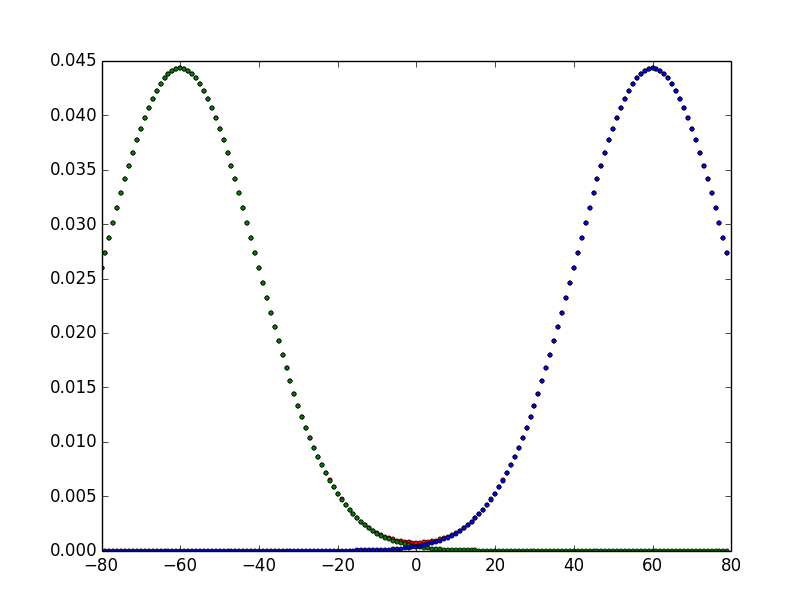
\includegraphics[scale=0.5]{gauss.png} 
\end{figure} 
 

\end{document}


